\section{Graph Convolutional Networks}

\begin{itemize}
  \item Idee: setze $k = 2$ für alle Faltungsebenen
  \item Begründung: $k < 2$ berücksichtigt nur alle Knoten, die zum jeweiligen Faltungsknoten adjazent sind
  \item für CNNs hat sich gezeigt, dass kleine Filtergrößen wie $3 \times 3$ keine negativen Auswirkungen haben
  \item viele kleine Faltungsebenen ohne Pooling propagieren die Informationen weit entfernterer Knoten weiter \todo{VGG Paper, oder he et al, deep residual learning}
  \item kann das Problem des Overfitting reduzieren für Graphen mit hohem Grad
\end{itemize}

Annahme: $\lambda_{\max} \approx 2$ \todo{ist das begründet, woher kommt diese Zahl}
Begründung: Netzparameter werden die Veränderung der Skalierung von $\mathbf{\tilde L}$ annehmen/ausgleichen.
Dann ist $\mathbf{\tilde L} = \mathbf{L} - \mathbf{I}$.

Dann gilt für die Filterung eines Signals $\mathbf{x}$ über $g_{\mathbf{\theta}}$
\begin{equation}
  g_{\mathbf{\theta}} \star \mathbf{x} = \mathbf{U}g_{\mathbf{\theta}}\left(\mathbf{\Lambda}\right)\mathbf{U}^{\top}\mathbf{x} \approx g^{\prime}_{\mathbf{\theta^{\prime}}} \left(\mathbf{L}\right) \mathbf{x} = \sum_{i=0}^{k-1} \mathbf{\theta}^{\prime}_i T_i \left(\mathbf{L} - \mathbf{I}\right) \mathbf{x} = \mathbf{\theta}^{\prime}_0 \mathbf{x} + \mathbf{\theta}^{\prime}_1 \left(\mathbf{L} - \mathbf{I}\right) \mathbf{x}
\end{equation}
Wenn wir den normalisierten Laplacian benutzen, gegeben durch $\mathbf{L} = \mathbf{I} - \mathbf{D}^{-\frac{1}{2}} \mathbf{A} \mathbf{D}^{-\frac{1}{2}}$, dann lässt sich weiter vereinfachen mit
\begin{equation}
  g_{\mathbf{\theta}} \star \mathbf{x} \approx \mathbf{\theta}^{\prime}_0 \mathbf{x} - \mathbf{\theta}^{\prime}_1 \mathbf{D}^{-\frac{1}{2}} \mathbf{A} \mathbf{D}^{-\frac{1}{2}} \mathbf{x}
\end{equation}
Um die Gefahr des Overfittings und die Anzahl an Berechnungen weiter zu reduzieren, können die Anzahl der Parameter weiter reduziert werden.
Mit $\mathbf{\theta} = \mathbf{\theta}^{\prime}_0 = - \mathbf{\theta}^{\prime}_1$ gilt dann
\begin{equation}
  g_{\mathbf{\theta}} \star \mathbf{x} \approx \mathbf{\theta} \left(\mathbf{I} + \mathbf{D}^{-\frac{1}{2}} \mathbf{A} \mathbf{D}^{-\frac{1}{2}}\right) \mathbf{x}
\end{equation}

$\mathbf{I} + \mathbf{D}^{-\frac{1}{2}} \mathbf{A} \mathbf{D}^{-\frac{1}{2}}$ hat nun Eigenwerte im Bereich $\left[0, 2\right]$\todo{warum?}.
Wiederholte Anwendungen dieses Operators können daher zu numerischen Instabilitäten und dann zu explodierenden oder verschwindenen Gradienten führen.\todo{warum}
Um dies zu verhindern, wird folgende Renormalisierung vorgenommen:
$\mathbf{I} + \mathbf{D}^{-\frac{1}{2}} \mathbf{A} \mathbf{D}^{-\frac{1}{2}} \to \mathbf{\tilde D}^{-\frac{1}{2}} \mathbf{\tilde A} \mathbf{\tilde D}^{-\frac{1}{2}}$ mit $\mathbf{\tilde A} = \mathbf{A} + \mathbf{I}$ und $\mathbf{\tilde D}$ ist nun die Gradmatrix der renormalisierten Adjazenzmatrix $\mathbf{\tilde A}$.
\begin{equation}
  g_{\mathbf{\theta}} \star \mathbf{x} \approx \mathbf{\theta} \left(\mathbf{\tilde D}^{-\frac{1}{2}} \mathbf{\tilde A} \mathbf{\tilde D}^{-\frac{1}{2}}\right) \mathbf{x}
\end{equation}

\begin{equation}
  H^{(l+1)} = f(H^{(l)}, A)
\end{equation}

\begin{equation}
  f(H^{(l)}, A) = \sigma(AH^{(l)}W^{(l)})
\end{equation}

\begin{equation}
  D_{ii} = \sum_j A_{ij}
\end{equation}

Für die Potenz $x \in \gls{R}$ einer Diagonalmatrix $D \in \gls{R}^{N \times N}$ gilt:

\begin{equation}
  D^x = \begin{pmatrix}
    d_{11} & 0 & \cdots & 0\\
    0 & d_{22} & \cdots & 0\\
    \vdots & \vdots & \ddots & \vdots\\
    0 & 0 & \cdots & d_{nn}\\
  \end{pmatrix}^x = \begin{pmatrix}
    d_{11}^x & 0 & \cdots & 0\\
    0 & d_{22}^x & \cdots & 0\\
    \vdots & \vdots & \ddots & \vdots\\
    0 & 0 & \cdots & d_{nn}^x\\
  \end{pmatrix}
\end{equation}

\section{Erweiterung für mehrere Kantenattribute}

Graph Convolutional Networks berücksichtigen nur eine Adjazenzmatrix.
Das bedeutet insbesondere, dass ein Graph nur über ein Kantenattribut verfügen kann.
Das ist für ungewichtete Graphen die Markierung einer Kante ($a_{ij} \in \lbrace 0, 1 \rbrace$) oder für gewichte Graphen das Gewicht einer Kante ($a_{ij} \in \gls{R+}$).
Eine Menge von Kantenattributen kann über mehrere Adjazenzmatrizen definiert werden.
Damit ist es ebenfalls möglich unterschiedliche Kanten für unterschiedliche Attribute zu definieren.

Eine Menge von Adjazenzmatrizen $\mathcal{A} = \lbrace A_1, A_2, \ldots, A_m \rbrace$ mit $A_i \in \gls{R}^{n \times n}$ beschreibt damit eine Menge von $m$ Graphen über der gleichen Knotenmenge $\mathcal{V}$ mit Kardinalität $n$.

$\mathcal{A} \in \gls{R}^{m \times n \times n}$ kann zu einer zweidimensionalen Matrix $A \in \gls{R}^{m \cdot n \times n}$ geglättet werden.

Dann ist $A \cdot H^{(l)} \in \gls{R}^{m \cdot n \times d}$.
Reshape zu $\gls{R}^{n \times m \cdot d}$ und Gewichtsmatrix $G \in \gls{R}^{m \cdot d \times x}$.

\begin{equation}
  H^{(l+1)} = f(H^{(l)}, \mathcal{\tilde A}) = \sigma \left( \frac{1}{|\mathcal{\tilde A}|} \sum_{\tilde A_i \in \mathcal{\tilde A}} \tilde D_i^{-\frac{1}{2}} \tilde A_i \tilde D_i^{-\frac{1}{2}} H^{(l)} W^{(l)}_i \right)
\end{equation}

$\sigma(\cdot)$ kennzeichnet eine Aktivierungsfunktion wie zum Beispiel $\text{ReLU}(\cdot) = \max(0, \cdot)$.

\subsection{Übertragung auf räumlich eingebettete Graphen}

Graphknoten haben im Allgemeinen keine Position oder Lage im Raum.
Knoten, die Regionen in einer vorhandenen Segmentierung darstellen, haben jedoch offensichtlich eine gewisse Lage im Raum, die zum Beispiel über das Zentrum der Region definiert werden kann.
Diese Information ist vorhanden und wichtig und sollte demnach auch nicht verloren gehen.
Anstatt diese lokal im Knoten zu speichern, bietet es sich eher an diese Information in den Kanten zu speichern um eine bessere Faltung zu garantieren.
Die euklische Distanz zwischen zwei benacharten Regionszentren wahrt zwar die Information der Distanz zweier Knoten zueinander, verliert aber die Information der Position zweier Knoten zueinander.
Es bietet sich daher an, die horizontalen und vertikalen Abstände in einer Koordinate an den Kanten zu speichern.
Es ist zu beachten, dass wir dadurch zu einem gerichteten Graphen übergehen, bei dem jede Kante von $v$ nach $w$ auch eine Kante von $w$ nach $v$ besitzt.

Wir haben damit zwei Adjazenzmatrizen.
Da Graph Convolutional Networks nicht mit negativen Gewichten funktionieren, müssen wir negative Koordinaten in eine weitere Adjazenzmatrix schreiben.
Wir gelangen damit zu vier Adjazenzmatrizen, die die Verbindungen von einem Knoten beschreibt, die links, rechts, oben oder unten zu ihm liegen.
Wir definieren diese Adjazenzmatrizen respektive als $A_{\text{links}}, A_{\text{rechts}}, A_{\text{oben}}$ und $A_{\text{unten}}$ (vgl. Abbildung~\ref{adjazenz_aufteilung}).
Falls eine Kante horizontal bzw.\ vertikal liegt, so definieren wir $a_{ij} = 1$ respektive für beide \glqq{}gegenüberliegenden\grqq\ Adjazenzmatrizen.

\begin{figure}
  \centering
  \subcaptionbox{$\mathcal{A}$}
  [\textwidth]{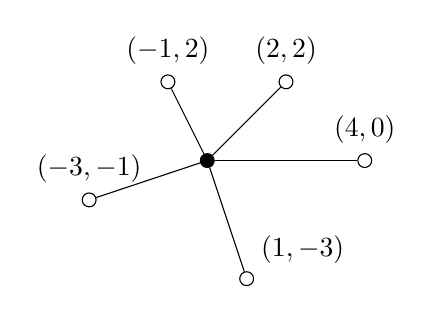
\begin{tikzpicture}
    \tikzstyle{node}=[circle,draw, minimum width=5pt, inner sep=0pt]
    \tikzstyle{root}=[fill=black]

    \node[node, root] (root) at (0,0) {};
    \node[node, label={$(-1, 2)$}] (a) at (-0.5, 1) {};
    \node[node, label={$(4, 0)$}] (b) at (2, 0) {};
    \node[node, label={$(2, 2)$}] (c) at (1, 1) {};
    \node[node, label={$(-3, -1)$}] (d) at (-1.5, -0.5) {};
    \node[node, label={50:$(1, -3)$}] (e) at (0.5, -1.5) {};

    \path (root) edge (a);
    \path (root) edge (b);
    \path (root) edge (c);
    \path (root) edge (d);
    \path (root) edge (e);
  \end{tikzpicture}
  }
  \subcaptionbox{$A_{\text{links}}$}
  [.2\textwidth]{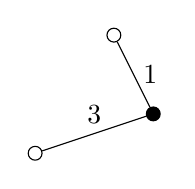
\begin{tikzpicture}
    \tikzstyle{node}=[circle,draw, minimum width=5pt, inner sep=0pt]
    \tikzstyle{root}=[fill=black]

    \node[node, root] (root) at (0,0) {};
    \node[node] (a) at (-0.5, 1) {};
    \node[node] (d) at (-1.5, -0.5) {};

    \path (root) edge[right] node {1} (a);
    \path (root) edge[above] node {3} (d);
  \end{tikzpicture}
  }
  \subcaptionbox{$A_{\text{rechts}}$}
  [.2\textwidth]{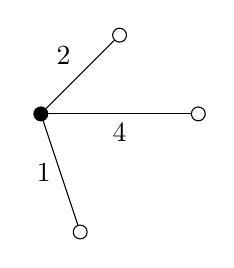
\begin{tikzpicture}
    \tikzstyle{node}=[circle,draw, minimum width=5pt, inner sep=0pt]
    \tikzstyle{root}=[fill=black]

    \node[node, root] (root) at (0,0) {};
    \node[node] (b) at (2, 0) {};
    \node[node] (c) at (1, 1) {};
    \node[node] (e) at (0.5, -1.5) {};

    \path (root) edge[below] node {4} (b);
    \path (root) edge[above left] node {2} (c);
    \path (root) edge[left] node {1} (e);
  \end{tikzpicture}
  }
  \subcaptionbox{$A_{\text{oben}}$}
  [.2\textwidth]{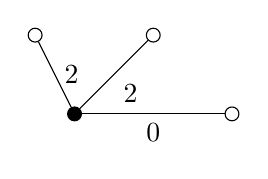
\begin{tikzpicture}
    \tikzstyle{node}=[circle,draw, minimum width=5pt, inner sep=0pt]
    \tikzstyle{root}=[fill=black]

    \node[node, root] (root) at (0,0) {};
    \node[node] (a) at (-0.5, 1) {};
    \node[node] (b) at (2, 0) {};
    \node[node] (c) at (1, 1) {};

    \path (root) edge[right] node {2} (a);
    \path (root) edge[below] node {0} (b);
    \path (root) edge[below right] node {2} (c);
  \end{tikzpicture}
  }
  \subcaptionbox{$A_{\text{unten}}$}
  [.2\textwidth]{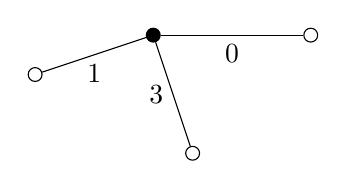
\begin{tikzpicture}
    \tikzstyle{node}=[circle,draw, minimum width=5pt, inner sep=0pt]
    \tikzstyle{root}=[fill=black]

    \node[node, root] (root) at (0,0) {};
    \node[node] (b) at (2, 0) {};
    \node[node] (d) at (-1.5, -0.5) {};
    \node[node] (e) at (0.5, -1.5) {};

    \path (root) edge[below] node {0} (b);
    \path (root) edge[below] node {1} (d);
    \path (root) edge[left] node {3} (e);
  \end{tikzpicture}
  }
\caption{Aufteilung einer Adjazenzmatrix in vier räumlich eingebettete Bereiche.}
\label{adjazenz_aufteilung}
\end{figure}

Kantenattribute bzw.\ Positionen von Knoten sollten skalierungsinvariant gespeichert werden.
Dafür werden die Abstände auf den Einheitskreis gemappt, wobei der Knoten mit der längsten Distanz zum Wurzelknoten genau auf dem Einheitskreis liegt (vgl. Abbildung~\ref{einheitskreis}).

\begin{figure}
\begin{tikzpicture}
  \draw[dashed] (0, 0) circle (4);

  \tikzstyle{node}=[circle,draw, minimum width=5pt, inner sep=0pt, fill=white]
  \tikzstyle{root}=[fill=black]

  \node[node, root] (root) at (0,0) {};
  \node[node, label={[fill=white]150:$(-1, 2) \rightarrow (-.25,.5)$}] (a) at (-1, 2) {};
  \node[node, label={[fill=white]$(4, 0) \rightarrow (1, 0)$}] (b) at (4, 0) {};
  \node[node, label={[fill=white]$(2, 2) \rightarrow (.5,.5)$}] (c) at (2, 2) {};
  \node[node, label={[fill=white]150:$(-3, -1) \rightarrow (-.75, -.25)$}] (d) at (-3, -1) {};
  \node[node, label={[fill=white]50:$(1, -3) \rightarrow (.25, -.75)$}] (e) at (1, -3) {};

  \path (root) edge (a);
  \path (root) edge (b);
  \path (root) edge (c);
  \path (root) edge (d);
  \path (root) edge (e);
\end{tikzpicture}
\caption{Abbildung der lokalen Nachbarschaftsknoten auf den Einheitskreis.}
\label{einheitskreis}
\end{figure}

Für die Anwendung auf das Graph Convolutional Network müssen die Gewichte aller Adjazenzmatrizen $a_{xij} \in [0, 1]$ invertiert werden, damit nähere Knoten einen größeren Einfluss haben.
Ebenso müssen \emph{Self Loops} für alle Knoten hinzugefügt werden.
Wir definieren unsere Adjazenzmatrix $\tilde A \in \mathbb{R}^{N \times N}$ aus einer Adjazenzmatrix $A \in \mathbb{R}^{N \times N}$ dann über

\begin{equation}
  \tilde A_{ij} = \begin{cases}
    1, & \text{falls }i=j\text{,}\\
    {(a_{ij}+1)}^{-1}, & \text{falls }a_{ij} \neq 0\text{,}\\
    0, & \text{sonst.}
  \end{cases}
\end{equation}

Dann ist $\tilde a_{ij} \in [1, 0.5]$

Diagonalmatrix ist schwierig.
Man will ja die Normalisierung damit $H^{(l)}$ nicht überskaliert.
Ich würde auch die gewichtete Matrix normalisieren.
Denke das macht Sinn.
Dann fallen die Werte ab, wenn viele Knoten weit entfernt sind.
